\documentclass[a4j, titlepage]{jarticle}

\usepackage[table,xcdraw]{xcolor}
\usepackage[dvipdfmx]{graphicx}
\usepackage{caption}
\usepackage{subcaption}
\usepackage{listings}
\usepackage{fancybox}
\usepackage{ascmac}
\usepackage{amsmath}
\usepackage{longtable}
\usepackage{subfig}

\definecolor{codegreen}{rgb}{0,0.6,0}
\definecolor{codegray}{rgb}{0.5,0.5,0.5}
\definecolor{codepurple}{rgb}{0.58,0,0.82}
\definecolor{backcolour}{rgb}{0.95,0.95,0.92}

% Define a custom style
\lstdefinestyle{mystyle}{
    backgroundcolor=\color{backcolour},   
    commentstyle=\color{codegreen},
    keywordstyle=\color{magenta},
    numberstyle=\tiny\color{codegray},
    stringstyle=\color{codepurple},
    basicstyle=\ttfamily\footnotesize,
    breakatwhitespace=false,         
    breaklines=true,                 
    captionpos=b,                    
    keepspaces=true,                 
    numbers=left,                    
    numbersep=5pt,                  
    showspaces=false,                
    showstringspaces=false,
    showtabs=false,                  
    tabsize=2,
    frame=single
}

\lstset{style=mystyle}

\begin{document}
  \begin{center}
  \huge 情報工学実験II\par
  \vspace{15mm}
  \huge テーマ02 \par
  \huge 乱数を用いたプログラム \par
  \vspace{15mm}
  % \LARGE タイトル \par
  \vspace{20mm}
  \vspace{100mm}
  \Large 令和5年07月06日 \par
  \vspace{15mm}
  \Large イマム カイリ ルビス \par
  \vspace{10mm}
  \Large 学籍番号:214071\par
  \vspace{10mm}
\end{center}
\clearpage

\tableofcontents
\clearpage

\section{概要}
  \subsection{乱数とは}
    乱数とは,ある数字の集合からランダムに選ばれた数字のことである.指定された分布内のすべての数値は,ランダムに選択される確率が等しくなります.

  \subsection{C言語の乱数関数}
    本実験のコードはすべてC言語で書かれている.C言語にはすでに乱数関数が用意されているので,本実験ではそれを利用する.

    \texttt{rand()}の関数は\texttt{stdlib.h}ヘッダーに含まれている.しかし,実行するたびに異なる乱数値を得るためには,\texttt{srand(time(NULL))}という関数も利用する必要がある.つまり,\texttt{time.h}ヘッダーファイルもインクルードする必要がある.\cite{cite:rand}

  \subsection{確率とは}
    確率とはある事象の確率は,その事象が起こる可能性を示す数値である.その事象が起こる可能性が高ければ高いほど,確率値は高くなる.\cite{cite:wiki}
  
    確率の基本的な計算は次の公式で計算される.
    \begin{screen}
      \begin{equation}
        P(A) = \frac{f}{N}
      \end{equation}
    \end{screen}
    事象Aが発生する確率を$P(A)$,事象Aが発生する可能性の数を$f$,可能な結果の合計数$N$.

  \subsection{実行環境}
    本実験で使用される実行環境:
    \begin{screen}
        \begin{itemize}
            \item プロセッサ:AMD Ryzen 5 5600X
            \item メモリー:16.0 GB
            \item OS:Windows 11 Pro
            \item コンパイラ:gcc
        \end{itemize}    
    \end{screen}

  \section{課題1:7個のサイコロを同じ出目になる確率}
  7個のサイコロを一緒に振って,すべてのサイコロが同じ出目になる確率を計算する課題である.しかし,結果に変化を与えるために,4面サイコロ,5面サイコロ,6面サイコロの確率を計算してみた.

  \subsection{同じ出目になる確率の理論値}
    同じ出目になる確率は以下の公式で計算することができる.
    \begin{screen}
      \begin{equation}
        P =  \left(\frac{1}{n}\right)^m \times n
      \end{equation}
    \end{screen}
    サイコロの面の数を$n$,サイコロの数を$m$とする.

    したがって,各サイコロ類の同じ出目になる確率は以下になる.
    \begin{itembox}[l]{4面サイコロ}
      \begin{align}
        P &=  \left(\frac{1}{4}\right)^7 \times 4 \nonumber \\
        P &= \frac{1}{4096} \nonumber \\
        P &= 2.4414 \times 10^{-4} \nonumber\\
        P &= 0.024414\%
      \end{align}
    \end{itembox}
    \begin{itembox}[l]{5面サイコロ}
      \begin{align}
        P &=  \left(\frac{1}{5}\right)^7 \times 5 \nonumber \\
        P &= \frac{1}{15625} \nonumber \\
        P &= 6.4 \times 10^{-5} \nonumber\\
        P &= 0.006400 \% 
      \end{align}
    \end{itembox}
    \begin{itembox}[l]{6面サイコロ}
      \begin{align}
        P &=  \left(\frac{1}{6}\right)^7 \times 6 \nonumber \\
        P &= \frac{1}{46656} \nonumber \\
        P &= 2.1433 \times 10^{-5} \nonumber \\
        P &= 0.002143\%
      \end{align}
    \end{itembox}

  \subsection{7個のサイコロのシミュレーションプログラム}
    以下は7個のサイコロをシミュレーションするプログラムである.
    \lstinputlisting[language=c]{D:/Kosen/jikkenII/random/Dir_Dice/dice.c} 
  
  \subsection{7個のサイコロのシミュレーションの流れ}
    サイコロの目がすべて一致するかどうかを確認する手順は以下の通りになる.
    \begin{screen}
      \begin{enumerate}
        \item 最初のサイコロを条件とする.
        \item 2個目から7個目まで順次に条件を満たすかどうかをチェックする.
        \item 全てのさいころが条件を満たしていれば成功.
        \item 条件を満たさないサイコロを1個でも見つければ,チェック処理を中断する.
      \end{enumerate}
    \end{screen}
  
  \subsection{7個のサイコロのシミュレーション結果}
    各サイコロ類について,最大$10^8$の反復で$3$回シミュレーションを行った.
    \subsubsection{4面サイコロのシミュレーション結果}
      以下は4面サイコロのシミュレーション結果である.
      \begin{longtable}[c]{|l|r|r|r|r|r|r|}
        \caption{4面サイコロのシミュレーション結果}
        \label{tab:dice4}\\
        \hline
        \rowcolor[HTML]{C0C0C0} 
        Count    & Probability\_1 & Error\_1 & Probability\_2 & Error\_2 & Probability\_3 & Error\_3 \\ \hline
        \endfirsthead
        %
        \endhead
        %
        $10^1$  & 0.000000\%     & 100.00\%         & 0.000000\%     & 100.00\%         & 0.000000\%     & 100.00\%         \\ \hline
        $10^2$  & 0.000000\%     & 100.00\%         & 0.000000\%     & 100.00\%         & 0.000000\%     & 100.00\%         \\ \hline
        $10^3$  & 0.000000\%     & 100.00\%         & 0.000000\%     & 100.00\%         & 0.100000\%     & 309.60\%         \\ \hline
        $10^4$  & 0.040000\%     & 63.84\%          & 0.010000\%     & 59.04\%          & 0.040000\%     & 63.84\%          \\ \hline
        $10^5$  & 0.016000\%     & 34.46\%          & 0.030000\%     & 22.88\%          & 0.027000\%     & 10.59\%          \\ \hline
        $10^6$  & 0.024300\%     & 0.47\%           & 0.025000\%     & 2.40\%           & 0.027300\%     & \cellcolor[HTML]{FD6864}11.82\%          \\ \hline
        $10^7$  & 0.025030\%     & 2.52\%           & 0.024360\%     & 0.22\%           & 0.024500\%     & 0.35\%           \\ \hline
        $10^8$  & 0.024524\%     & 0.45\%           & 0.024372\%     & 0.17\%           & 0.024659\%     & 1.00\%           \\ \hline
      \end{longtable}

      グラフで表すと以下のグラフになる.

      \begin{figure}[htb]
        % \centering
        % \hfill
        \begin{subfigure}[b]{0.38\textwidth}
            \centering
            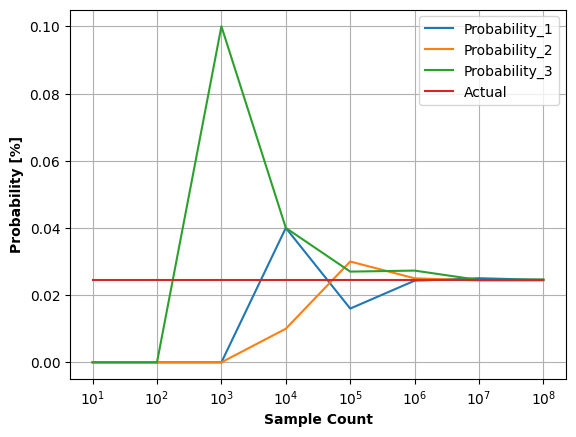
\includegraphics[height=\textwidth]{../Dir_Dice/img_result4.png}
            % \centering
            \captionsetup{justification=centering, singlelinecheck=false, margin={70pt,0pt}}
            \caption{確率値}
            \label{fig:dic4}
        \end{subfigure}
        \hspace{50pt}
        \begin{subfigure}[b]{0.38\textwidth}
          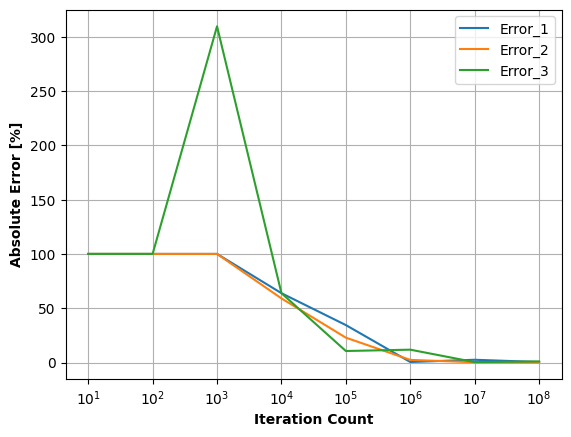
\includegraphics[height=\textwidth]{../Dir_Dice/img_error4.png}
          \captionsetup{justification=centering, singlelinecheck=false, margin={70pt,0pt}}
          \caption{絶対誤差}
          \label{fig:errdic4}
        \end{subfigure}
        \hfill
            \caption{4面サイコロの確率値と絶対誤差}
           \label{fig:resdic4}
      \end{figure}
    
      \subsubsection{5面サイコロのシミュレーション結果}
        以下は5面サイコロのシミュレーション結果である.

        \begin{longtable}[c]{|l|r|r|r|r|r|r|}
          \caption{5面サイコロのシミュレーション結果}
          \label{tab:dice5}\\
          \hline
          \rowcolor[HTML]{C0C0C0} 
          Count    & Probability\_1 & Error\_1 & Probability\_2 & Error\_2 & Probability\_3 & Error\_3 \\ \hline
          \endfirsthead
          %
          \endhead
          %
          $10^1$   & 0.000000\%     & 100.00\%         & 0.000000\%     & 100.00\%         & 0.000000\%     & 100.00\%         \\ \hline
          $10^2$   & 0.000000\%     & 100.00\%         & 0.000000\%     & 100.00\%         & 0.000000\%     & 100.00\%         \\ \hline
          $10^3$   & 0.000000\%     & 100.00\%         & 0.000000\%     & 100.00\%         & 0.000000\%     & 100.00\%         \\ \hline
          $10^4$   & 0.010000\%     & 56.25\%          & 0.000000\%     & 100.00\%         & 0.020000\%     & 212.50\%         \\ \hline
          $10^5$   & 0.007000\%     & 9.38\%           & 0.005000\%     & 21.88\%          & 0.006000\%     & 6.25\%           \\ \hline
          $10^6$   & 0.007900\%     & \cellcolor[HTML]{FD6864}23.44\%          & 0.006100\%     & 4.69\%           & 0.006500\%     & 1.56\%           \\ \hline
          $10^7$   & 0.006490\%     & 1.41\%           & 0.006430\%     & 0.47\%           & 0.006340\%     & 0.94\%           \\ \hline
          $10^8$   & 0.006547\%     & 2.30\%           & 0.006403\%     & 0.05\%           & 0.006529\%     & 2.02\%           \\ \hline
        \end{longtable}
        
        グラフで表すと以下のグラフになる.

        \begin{figure}[htb]
          % \centering
          % \hfill
          \begin{subfigure}[b]{0.38\textwidth}
              \centering
              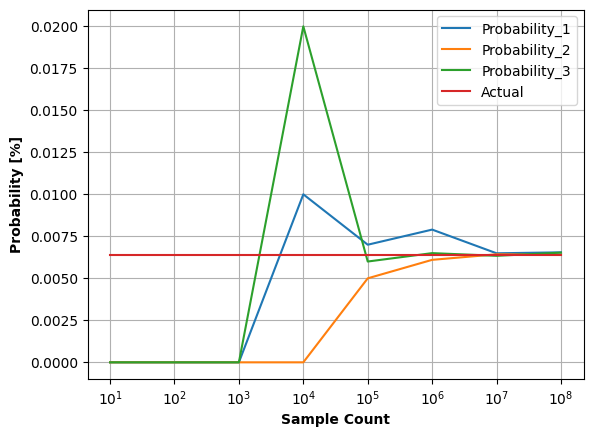
\includegraphics[height=\textwidth]{../Dir_Dice/img_result5.png}
              % \centering
              \captionsetup{justification=centering, singlelinecheck=false, margin={80pt,0pt}}
              \caption{確率値}
              \label{fig:dic5}
          \end{subfigure}
          \hspace{50pt}
          \begin{subfigure}[b]{0.38\textwidth}
            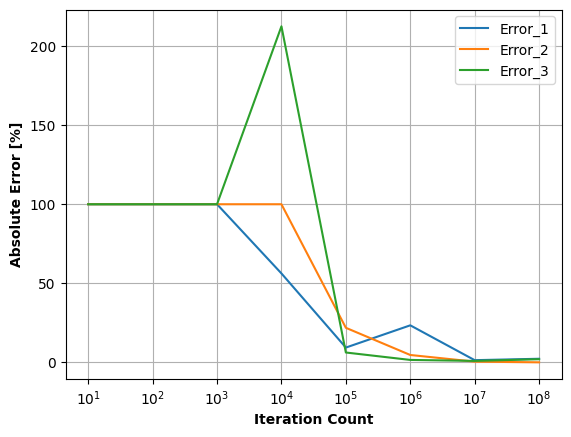
\includegraphics[height=\textwidth]{../Dir_Dice/img_error5.png}
            \captionsetup{justification=centering, singlelinecheck=false, margin={70pt,0pt}}
            \caption{絶対誤差}
            \label{fig:errdic5}
          \end{subfigure}
          \hfill
              \caption{5面サイコロの確率値と絶対誤差}
             \label{fig:resdic5}
        \end{figure}
      
      \subsubsection{6面サイコロのシミュレーション結果}
        以下は6面サイコロのシミュレーション結果である.

        \begin{longtable}[c]{|l|r|r|r|r|r|r|r|}
          \caption{6面サイコロのシミュレーション結果}
          \label{tab:dice6}\\
          \hline
          \rowcolor[HTML]{C0C0C0} 
          Count    & Probability\_1 & Error\_1 & Probability\_2 & Error\_2 & Probability\_3 & Error\_3 \\ \hline
          \endfirsthead
          %
          \endhead
          %
          $10^1$    & 0.000000\%     & 100.000\%        & 0.000000\%     & 100.000\%        & 0.000000\%     & 100.000\%        \\ \hline
          $10^2$    & 0.000000\%     & 100.000\%        & 0.000000\%     & 100.000\%        & 0.000000\%     & 100.000\%        \\ \hline
          $10^3$    & 0.000000\%     & 100.000\%        & 0.000000\%     & 100.000\%        & 0.000000\%     & 100.000\%        \\ \hline
          $10^4$    & 0.000000\%     & 100.000\%        & 0.000000\%     & 100.000\%        & 0.000000\%     & 100.000\%        \\ \hline
          $10^5$    & 0.004000\%     & 86.624\%         & 0.002000\%     & 6.688\%          & 0.005000\%     & 133.280\%        \\ \hline
          $10^6$    & 0.001500\%     & \cellcolor[HTML]{FD6864}30.016\%         & 0.002000\%     & \cellcolor[HTML]{FD6864}6.688\%          & 0.002500\%     & \cellcolor[HTML]{FD6864}16.640\%         \\ \hline
          $10^7$    & 0.002140\%     & 0.156\%          & 0.002160\%     & 0.777\%          & 0.002090\%     & 2.489\%          \\ \hline
          $10^8$    & 0.002139\%     & 0.203\%          & 0.002158\%     & 0.684\%          & 0.002146\%     & 0.124\%          \\ \hline
        \end{longtable}

      グラフで表すと以下のグラフになる.

      \begin{figure}[htb]
        % \centering
        % \hfill
        \begin{subfigure}[b]{0.38\textwidth}
            \centering
            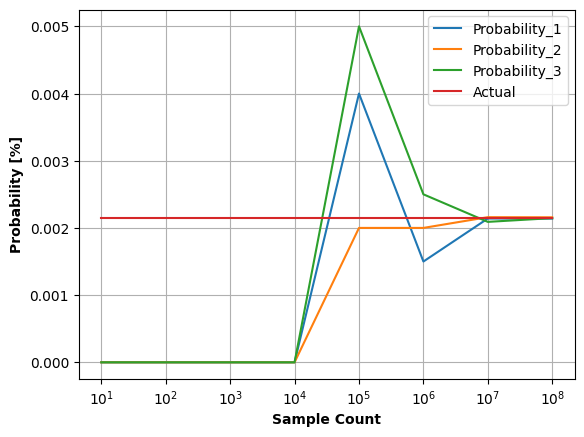
\includegraphics[height=\textwidth]{../Dir_Dice/img_result6.png}
            % \centering
            \captionsetup{justification=centering, singlelinecheck=false, margin={70pt,0pt}}
            \caption{確率値}
            \label{fig:dic6}
        \end{subfigure}
        \hspace{50pt}
        \begin{subfigure}[b]{0.38\textwidth}
          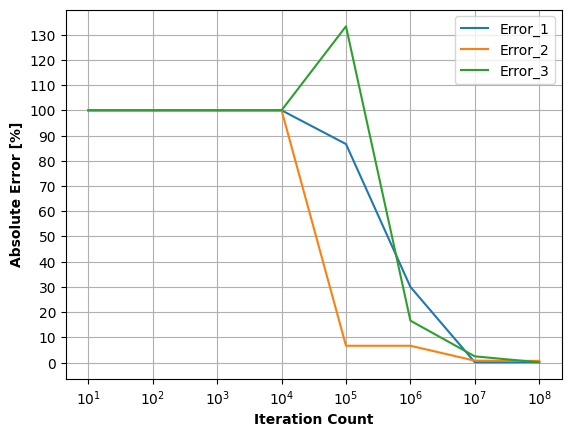
\includegraphics[height=\textwidth]{../Dir_Dice/img_error6.png}
          \captionsetup{justification=centering, singlelinecheck=false, margin={70pt,0pt}}
          \caption{絶対誤差}
          \label{fig:errdic6}
        \end{subfigure}
        \hfill
            \caption{6面サイコロの確率値と絶対誤差}
            \label{fig:resdic6}
      \end{figure}

    \subsection{7個のサイコロのシミュレーションの考察}
      4面サイコロ,5面サイコロ,6面サイコロのどのシミュレーションも,反復回数が増えるにつれて誤差が小さくなっています.図(1),図(2),図(3)を見ると,反復回数が$10^7$とき,全ての誤差が小さくなっていることがわかる.

      しかし,4面サイコロの1回目と2回目のシミュレーションでは,図(1(b))ように反復回数$10^6$のとき,誤差が小さくなるものもある.しかし,3回目のシミュレーションでは誤差が大きくなっている.同じことが5面サイコロでも起こり,反復回数が$10^6$最初のシミュレーションでは大きな誤差が出ました.最後の6面サイコロでは,誤差は小さくならなかった.つまり,正確な結果を得るためには,反復回数が$10^6$では十分ではないという結論になる.
  
  \section{課題2:円の面積}
    円の面積を計算するには,乱数によって点をプロットし,その点が円の中にあるかあるかどうかをを確認する.そして,四角形の面積と円の面積を比較する.計算過程は以下のようになる.
    \begin{screen}
      \begin{equation}
        \frac{円の面積}{四角形の面積} = \frac{a}{a+b} 
      \end{equation}
      \begin{equation}
        円の面積 = 四角形の面積 \times \frac{a}{a+b}
      \end{equation}
    \end{screen}
    円の内側の点の数を$a$,円の外側の点の数を$b$とする.

    \subsection{円の面積のシミュレーションプログラム}
      以下は7個のサイコロをシミュレーションするプログラムである.
      \lstinputlisting[language=c]{D:/Kosen/jikkenII/random/Dir_Area/area.c} 
    
    \subsection{円の面積のシミュレーションの流れ}
      サイコロの目がすべて一致するかどうかを確認する手順は以下の通りになる.
      \begin{screen}
        \begin{enumerate}
          \item 乱数によって点をプロットする.
          \item 円の内側と外側にプロットされている点を数える.
          \item 円の面積と四角形を比較して,円の面積を得る.
        \end{enumerate}
      \end{screen}

    \subsection{円の面積のシミュレーション結果}
      本実験で計算された円の半径は$7m$と$10m$とする.各円の半径の大きさに分れて,最大$10^8$の反復で$3$回シミュレーションを行った.

      \subsubsection{半径$7m$の円のシミュレーション結果}
        以下は半径$7m$の円のシミュレーション結果である.

        \begin{longtable}[c]{|r|r|r|r|r|r|r|}
          \caption{半径$7m$の円のシミュレーション結果}
          \label{tab:area7}\\
          \hline
          \rowcolor[HTML]{C0C0C0} 
          Sample Count    & Result\_1 [$m^2$] & Error\_1 & Result\_2 [$m^2$] & Error\_2 & Result\_3 [$m^2$] & Error\_3 \\ \hline
          \endfirsthead
          %
          \endhead
          %
          $10^1$    & 137.200   & 10.873\% & 156.800   & 1.859\%  & 117.600   & 23.606\% \\ \hline
          $10^2$    & 154.840   & 0.586\%  & 150.920   & 1.961\%  & 158.760   & 3.132\%  \\ \hline
          $10^3$    & 155.820   & 1.223\%  & 152.096   & 1.197\%  & 158.172   & 2.750\%  \\ \hline
          $10^4$    & 154.095   & 0.102\%  & 153.782   & 0.102\%  & 153.625   & 0.203\%  \\ \hline
          $10^5$    & 154.193   & 0.166\%  & 153.688   & 0.163\%  & 153.787   & 0.098\%  \\ \hline
          $10^6$    & 153.940   & 0.001\%  & 154.009   & 0.046\%  & 153.879   & 0.038\%  \\ \hline
          $10^7$    & 153.907   & 0.020\%  & 153.901   & 0.024\%  & 153.870   & 0.044\%  \\ \hline
          $10^8$    & 153.907   & 0.020\%  & 153.903   & 0.023\%  & 153.890   & 0.031\%  \\ \hline
        \end{longtable}
        
        グラフで表すと以下のグラフになる.
        \begin{figure}[htb]
          % \centering
          % \hfill
          \begin{subfigure}[b]{0.38\textwidth}
              \centering
              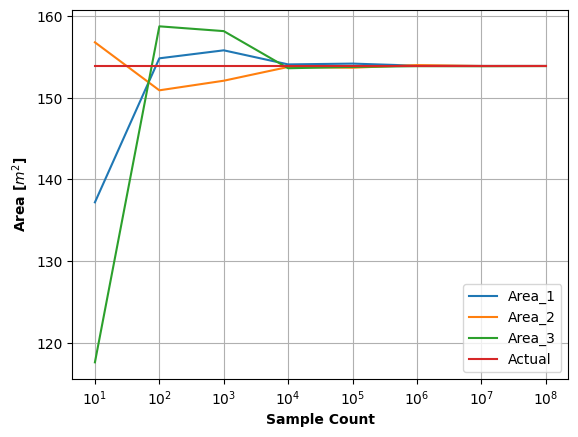
\includegraphics[height=\textwidth]{../Dir_Area/img_area7.png}
              \captionsetup{justification=centering, singlelinecheck=false, margin={70pt,0pt}}
              \caption{面積}
              \label{fig:area7}
          \end{subfigure}
          \hspace{50pt}
          \begin{subfigure}[b]{0.38\textwidth}
            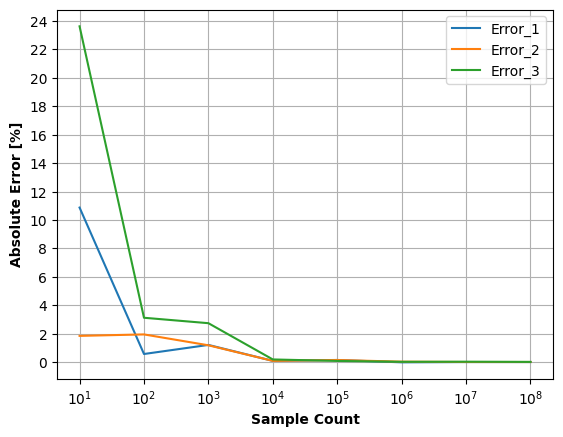
\includegraphics[height=\textwidth]{../Dir_Area/img_error7.png}
            \captionsetup{justification=centering, singlelinecheck=false, margin={70pt,0pt}}
            \caption{絶対誤差}
            \label{fig:errarea7}
          \end{subfigure}
          \hfill
              \caption{半径$7m$の円の面積と絶対誤差}
              \label{fig:resarea7}
        \end{figure}

      \vspace{20pt}
      \subsubsection{半径$10m$の円のシミュレーション結果}
        以下は半径$10m$の円のシミュレーション結果である.

        \begin{longtable}[c]{|r|r|r|r|r|r|r|}
          \caption{半径$10m$の円のシミュレーション結果}
          \label{tab:area10}\\
          \hline
          \rowcolor[HTML]{C0C0C0} 
          Sample Count   & Result\_1 & Error\_1 & Result\_2 & Error\_2 & Result\_3 & Error\_3 \\ \hline
          \endfirsthead
          %
          \endhead
          %
          $10^1$  & 280.000   & 10.873\% & 360.000   & 14.592\% & 240.000   & 23.606\% \\ \hline
          $10^2$  & 332.000   & 5.679\%  & 332.000   & 5.679\%  & 324.000   & 3.132\%  \\ \hline
          $10^3$  & 321.200   & 2.241\%  & 307.200   & 2.215\%  & 314.800   & 0.204\%  \\ \hline
          $10^4$  & 314.360   & 0.064\%  & 312.480   & 0.535\%  & 313.360   & 0.254\%  \\ \hline
          $10^5$  & 313.804   & 0.113\%  & 314.480   & 0.102\%  & 314.840   & 0.217\%  \\ \hline
          $10^6$  & 314.026   & 0.042\%  & 314.402   & 0.077\%  & 314.145   & 0.004\%  \\ \hline
          $10^7$  & 314.149   & 0.003\%  & 314.104   & 0.018\%  & 314.139   & 0.006\%  \\ \hline
          $10^8$  & 314.144   & 0.005\%  & 314.168   & 0.003\%  & 314.168   & 0.003\%  \\ \hline
        \end{longtable}

        グラフで表すと以下のグラフになる.
        \begin{figure}[htb]
          % \centering
          % \hfill
          \begin{subfigure}[b]{0.38\textwidth}
              \centering
              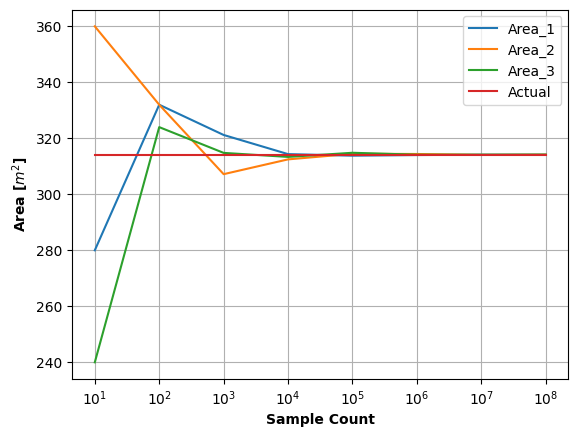
\includegraphics[height=\textwidth]{../Dir_Area/img_area10.png}
              \captionsetup{justification=centering, singlelinecheck=false, margin={70pt,0pt}}
              \caption{面積}
              \label{fig:area10}
          \end{subfigure}
          \hspace{50pt}
          \begin{subfigure}[b]{0.38\textwidth}
            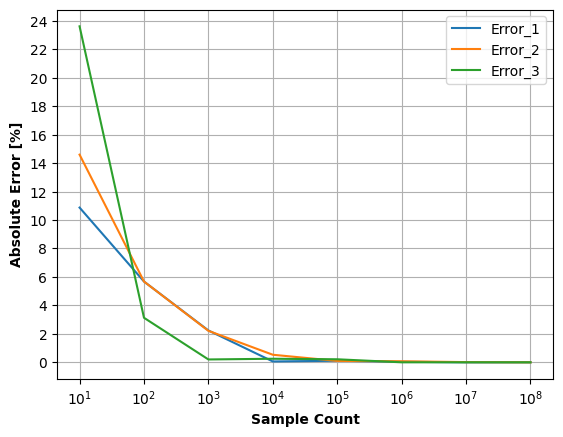
\includegraphics[height=\textwidth]{../Dir_Area/img_error10.png}
            \captionsetup{justification=centering, singlelinecheck=false, margin={70pt,0pt}}
            \caption{絶対誤差}
            \label{fig:errarea10}
          \end{subfigure}
          \hfill
              \caption{半径$10m$の円の面積と絶対誤差}
              \label{fig:resarea10}
        \end{figure}
        % \clearpage
      
      \subsection{円の面積のシミュレーションの考察}
        図(\ref{fig:resarea7})と図(\ref{fig:resarea10})からシミュレーションの結果は,サンプル数が増えるにつれて,より正確になっていくことがわかる.サンプル数が$10^4$のとき,絶対誤差が$1\%$未満になる.サンプル数を$10^6$ポイントでシミュレーションを行うと,誤差は$0.1\%$以下になる.しかし,サンプルをそれ以上に増やしても,誤差は有意な減少を示さない.

        したがって,作業負荷と精度を考慮すると,$10^6$ サンプルを使用するのが最も効率的.つまり作業量が少なく精度が高い.

  \section{課題3:10名の男女横一列に並べる}
    女性5人と男性5人の計10人が横一列に並べる.順番は完全に乱数によって決まる.しかし,期待される並び方は,各女性に対して,自身より背の高い男性が左に少なくとも一人いる.ということ,この課題はこの並び方が起こった確率計算する課題である.
    
    \subsection{横一列に並べるシミュレーションプログラム}
      以下は10名を横一列に並べるをシミュレーションするプログラムである.
      \lstinputlisting[language=c]{D:/Kosen/jikkenII/random/Dir_Height/height.c} 

    
    
    \subsection{10名を横一列に並べるシミュレーションの流れ}
      乱数できめた並び方を確認する手順は以下の通りになる.
      \begin{screen}
        \begin{enumerate}
          \item 乱数で全員の位置を決定する.
          \item 各女性に左に立っている男性と身長を比較する.
          \item 条件を満たさない女性を1人でも見つければ,チェック処理を中断する.
        \end{enumerate}
      \end{screen}
    
    \subsection{10名を横一列に並べるの理論値}
      この問題で期待される条件の並び方が起こった確率を数学的に計算すると,次のようになる.
      \begin{screen}
        \begin{equation}
          P = \frac{1 \times 3 \times 5 \times 7 \times 9}{2 \times 4 \times 6 \times 8 \times 10}
        \end{equation}
        \begin{equation}
          P = 0.24609
        \end{equation}
        \begin{equation}
          P = 24.609375\%
        \end{equation}
      \end{screen}
    
    \subsection{10名を横一列に並べるシミュレーションの結果}
      この課題をシミュレーションを行うとき,最大$10^8$の反復で$3$回シミュレーションを行った.その結果は以下になる.

      \begin{longtable}[c]{|r|r|r|r|r|r|r|}
        \caption{10名を横一列に並べるシミュレーションの結果}
        \label{tab:height}\\
        \hline
        \rowcolor[HTML]{C0C0C0} 
        Count    & Probability\_1 & Error\_1 & Probability\_2 & Error\_2 & Probability\_3 & Error\_3 \\ \hline
        \endfirsthead
        %
        \endhead
        %
        $10^1$   & 20.000000\%      & 18.730\% & 30.000000\%      & 21.905\% & 20.000000\%      & 18.730\% \\ \hline
        $10^2$   & 19.000000\%      & 22.794\% & 27.000000\%      & 9.714\%  & 24.000000\%      & 2.476\%  \\ \hline
        $10^3$   & 24.800000\%      & 0.775\%  & 25.800000\%      & 4.838\%  & 25.500000\%      & 3.619\%  \\ \hline
        $10^4$   & 24.320000\%      & 1.176\%  & 23.910000\%      & 2.842\%  & 24.790000\%      & 0.734\%  \\ \hline
        $10^5$   & 24.726000\%      & 0.474\%  & 24.579000\%      & 0.123\%  & 24.592000\%      & 0.071\%  \\ \hline
        $10^6$   & 24.626300\%      & 0.069\%  & 24.551900\%      & 0.234\%  & 24.557400\%      & 0.211\%  \\ \hline
        $10^7$   & 24.626050\%      & 0.068\%  & 24.624070\%      & 0.060\%  & 24.589280\%      & 0.082\%  \\ \hline
        $10^8$   & 24.612748\%      & 0.014\%  & 24.611035\%      & 0.007\%  & 24.608419\%      & 0.004\%  \\ \hline
      \end{longtable}

      \clearpage
      グラフで表すと以下のグラフになる.
      \begin{figure}[htb]
        % \centering
        % \hfill
        \begin{subfigure}[b]{0.38\textwidth}
            \centering
            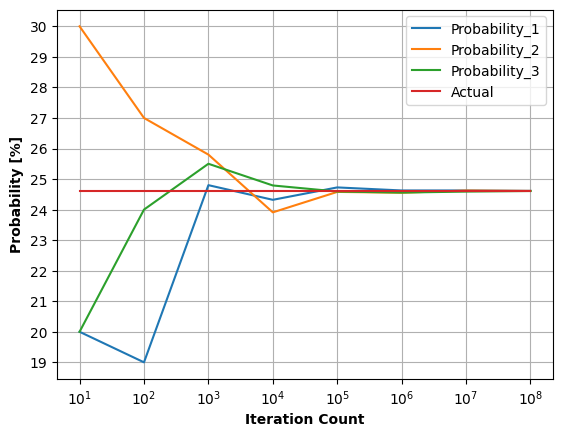
\includegraphics[height=\textwidth]{../Dir_Height/img_height.png}
            \captionsetup{justification=centering, singlelinecheck=false, margin={70pt,0pt}}
            \caption{確率値}
            \label{fig:height}
        \end{subfigure}
        \hspace{50pt}
        \begin{subfigure}[b]{0.38\textwidth}
          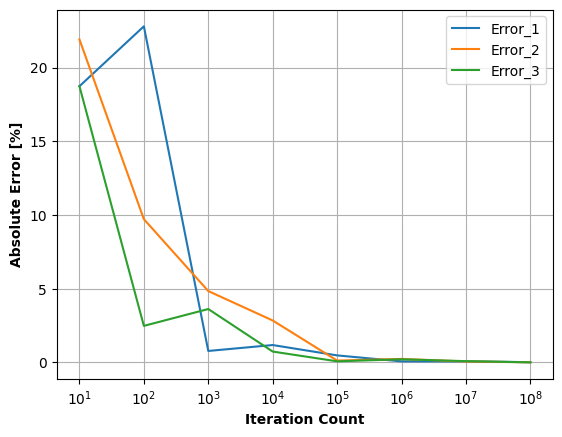
\includegraphics[height=\textwidth]{../Dir_Height/img_error.png}
          \captionsetup{justification=centering, singlelinecheck=false, margin={70pt,0pt}}
          \caption{絶対誤差}
          \label{fig:errheight}
        \end{subfigure}
        \hfill
            \caption{10名の男女横一列に並べる確率}
            \label{fig:resheight}
      \end{figure}

    \subsection{10名を横一列に並べるシミュレーションの考察}
      表(\ref{tab:height})をから見ると,最初にすべての絶対誤差が$0.1\%$未満になったのは,反復回数が$10^7$回のときである.つまり,この課題は$24.626\%$の確率で発生し,正確な結果を得るには$10^7$回のシミュレーションが必要という結論になる.

  \section{課題4:コインゲーム}
    サイコロを使ったゲームで,1か2の目が出るたびにBがAにコインを1枚渡し,それ以外出たらAがBにコインを1枚渡す.これを繰り返して,最後にコインを全部持っている方が勝つ.
    この課題では,Aがゲームに勝つ確率を計算することが目的である.
    
    \subsection{コインゲームのシミュレーションプログラム}
      以下はコインゲームをシミュレーションするプログラムである.
      \lstinputlisting[language=c]{D:/Kosen/jikkenII/random/Dir_Coin/coin.c} 
    
    \subsection{コインゲームのシミュレーション結果}
      Aのコインの枚数の違いによる影響を知るために,コインの枚数で分けて,シミュレーションを行った.各シミュレーションは3回行った.
      
      \subsubsection{Aが5枚コインで始まる}
        以下はAが5枚コインで始まったゲームのシミュレーション結果である.

        \begin{longtable}[c]{|r|r|r|r|}
          \caption{Aが5枚コインで始まる結果}
          \label{tab:coin5}\\
          \hline
          \rowcolor[HTML]{C0C0C0} 
          Count    & Probability\_1 & Probability\_2 & Probability\_3 \\ \hline
          \endfirsthead
          %
          \endhead
          %
          $10^1$   &  0.00000\%       & 20.00000\%       & 20.00000\%       \\ \hline
          $10^2$   & 15.00000\%       &  6.00000\%       & 13.00000\%       \\ \hline
          $10^3$   & 11.90000\%       & 11.90000\%       & 12.50000\%       \\ \hline
          $10^4$   & 11.60000\%       & 12.27000\%       & 12.52000\%       \\ \hline
          $10^5$   & 12.04900\%       & 12.06100\%       & 12.25900\%       \\ \hline
          $10^6$   & 12.16000\%       & 12.14950\%       & 12.14660\%       \\ \hline
          $10^7$   & 12.13316\%       & 12.15369\%       & 12.17129\%       \\ \hline
          $10^8$   & 12.16059\%       & 12.15940\%       & 12.15675\%       \\ \hline
        \end{longtable}

        グラフで表すと以下のグラフになる.
        \begin{figure}[htb]
          \begin{center}
            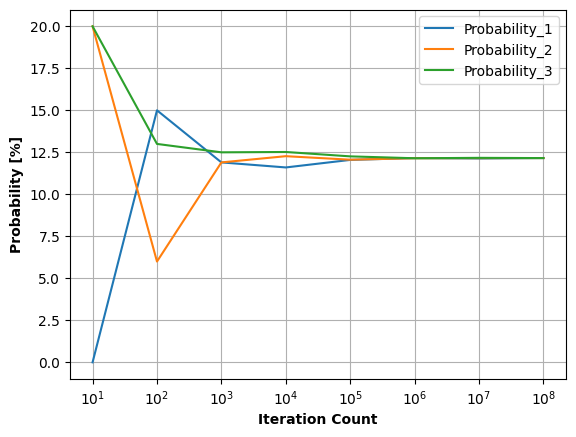
\includegraphics[scale=0.55]{../Dir_Coin/img_coin5.png}
            \caption{Aが5枚コインで始まった勝つ確率}
            \label{img:coin5}
          \end{center}
        \end{figure}

      \subsubsection{Aが6枚コインで始まる}
        以下はAが6枚コインで始まったゲームのシミュレーション結果である.

        \begin{longtable}[c]{|r|r|r|r|}
          \caption{Aが6枚コインで始まる結果}
          \label{tab:coin6}\\
          \hline
          \rowcolor[HTML]{C0C0C0} 
          count    & Probability\_1 & Probability\_2 & Probability\_3 \\ \hline
          \endfirsthead
          %
          \endhead
          %
          $10^1$   & 10.000000\%      & 30.000000\%      & 40.000000\%      \\ \hline
          $10^2$   & 20.000000\%      & 29.000000\%      & 21.000000\%      \\ \hline
          $10^3$   & 23.700000\%      & 24.900000\%      & 26.700000\%      \\ \hline
          $10^4$   & 25.450000\%      & 24.530000\%      & 24.890000\%      \\ \hline
          $10^5$   & 24.631000\%      & 24.569000\%      & 24.560000\%      \\ \hline
          $10^6$   & 24.606900\%      & 24.746600\%      & 24.748100\%      \\ \hline
          $10^7$   & 24.699580\%      & 24.708590\%      & 24.720960\%      \\ \hline
          $10^8$   & 24.712858\%      & 24.701537\%      & 24.711713\%      \\ \hline
        \end{longtable}

        グラフで表すと以下のグラフになる.
        \begin{figure}[htb]
          \begin{center}
            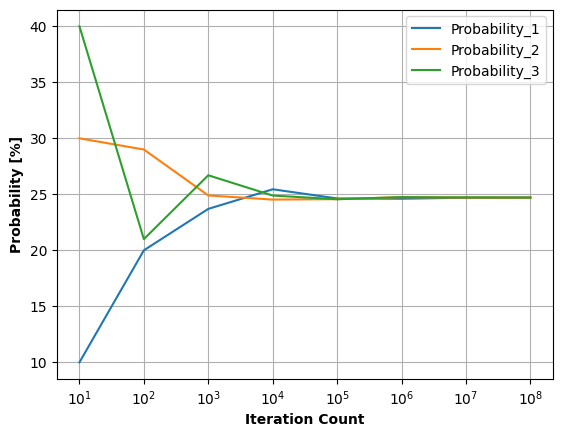
\includegraphics[scale=0.55]{../Dir_Coin/img_coin6.png}
            \caption{Aが6枚コインで始まった勝つ確率}
            \label{img:coin6}
          \end{center}
        \end{figure}
      
      \subsubsection{Aが7枚コインで始まる}
        以下はAが7枚コインで始まったゲームのシミュレーション結果である.

        \begin{longtable}[c]{|r|r|r|r|}
          \caption{Aが7枚コインで始まる結果}
          \label{tab:coin7}\\
          \hline
          \rowcolor[HTML]{C0C0C0} 
          count    & Probability\_1 & Probability\_2 & Probability\_3 \\ \hline
          \endfirsthead
          %
          \endhead
          %
          $10^1$   & 50.000000\%      & 40.000000\%      & 60.000000\%      \\ \hline
          $10^2$   & 51.000000\%      & 51.000000\%      & 52.000000\%      \\ \hline
          $10^3$   & 47.200000\%      & 50.700000\%      & 49.400000\%      \\ \hline
          $10^4$   & 50.200000\%      & 50.450000\%      & 49.400000\%      \\ \hline
          $10^5$   & 49.906000\%      & 49.861000\%      & 49.743000\%      \\ \hline
          $10^6$   & 49.863900\%      & 49.828300\%      & 49.811800\%      \\ \hline
          $10^7$   & 49.803250\%      & 49.803660\%      & 49.798380\%      \\ \hline
          $10^8$   & 49.809443\%      & 49.814332\%      & 49.802907\%      \\ \hline
        \end{longtable}
        \clearpage

        グラフで表すと以下のグラフになる.
        \begin{figure}[htb]
          \begin{center}
            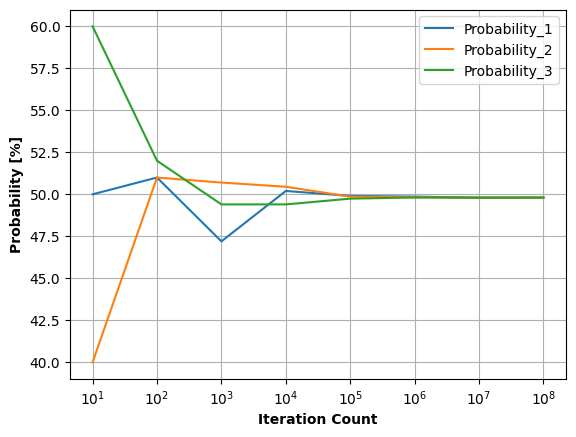
\includegraphics[scale=0.55]{../Dir_Coin/img_coin7.png}
            \caption{Aが7枚コインで始まった勝つ確率}
            \label{img:coin7}
          \end{center}
        \end{figure}
      
      \subsection{コインゲームの考察}
        表(\ref{tab:coin5}),表(\ref{tab:coin6}),表(\ref{tab:coin7})から見ると,コイン数が変わるとAが勝つ確率は以下のようになる.
        \begin{screen}
          \begin{itemize}
            \item Aが5枚コインで始まるかつ確率:$12.16\%$
            \item Aが6枚コインで始まるかつ確率:$24.70\%$
            \item Aが7枚コインで始まるかつ確率:$49.80\%$
          \end{itemize}
        \end{screen}
        Aが最初に持たせるコインの数が最大でも,Bがゲームに勝つ確率の方が高い.つまり,サイコロの目が1か2のときだけAにコインを出すという条件が,ゲームの勝率に最も大きな影響を与えていることがわかる.
    
    \section{課題5:ビンゴゲーム}
      この課題の目的は,ビンゴをシミュレートし,4回以内に当たる確率,7回以内に当たる確率,ビンゴゲームで起こる最大回数,最大回数が起こる確率を計算することである.

      ビンゴになるには,横・館・斜めのいずれか1列にある5マスが揃って有効になった場合に勝利となり.

      \subsection{ビンゴのシミュレーションプログラム}
        以下はコインゲームをシミュレーションするプログラムである.
        \lstinputlisting[language=c]{D:/Kosen/jikkenII/random/Dir_bingo_new/bingo.c} 
      
      \subsection{ビンゴのシミュレーションの流れ}
        ビンゴをシミュレートする手順は以下の通りになる.
        \begin{screen}
          \begin{enumerate}
            \item ビンゴカードを生成する.
            \item 乱数で番号をひき,ビンゴカードをチェックする.
            \item 横・館・斜めのいずれか1列にある5マスが揃うかどうかをチェックする.
            \item 揃っていない場合,2番に帰る.
          \end{enumerate}
        \end{screen}

      \subsection{ビンゴのシミュレーション結果}
        反復回数が$10^8$で3回のシミュレーションを行った.シミュレーション結果は以下のようになる.
        \clearpage

        \subsubsection{1回目のシミュレーション結果}
        1回目のシミュレーション結果をグラフで表すと以下のグラフになる.
        \begin{figure}[htb]
          \begin{center}
            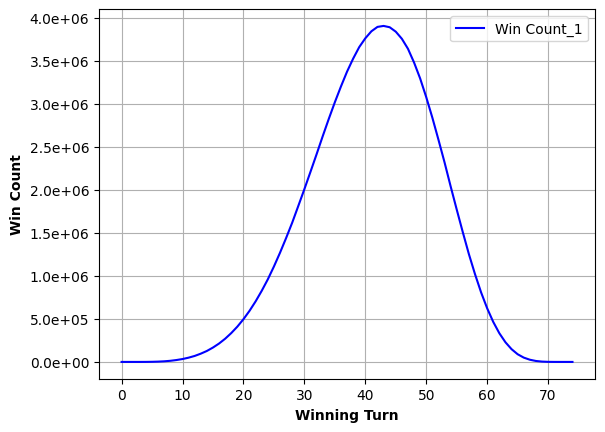
\includegraphics[scale=0.55]{../Dir_bingo_new/img_bingo1.png}
            \caption{1回目の当たる回数の分布}
            \label{img:bingo1}
          \end{center}
        \end{figure}

        \subsubsection{2回目のシミュレーション結果}
        2回目のシミュレーション結果をグラフで表すと以下のグラフになる.
        \begin{figure}[htb]
          \begin{center}
            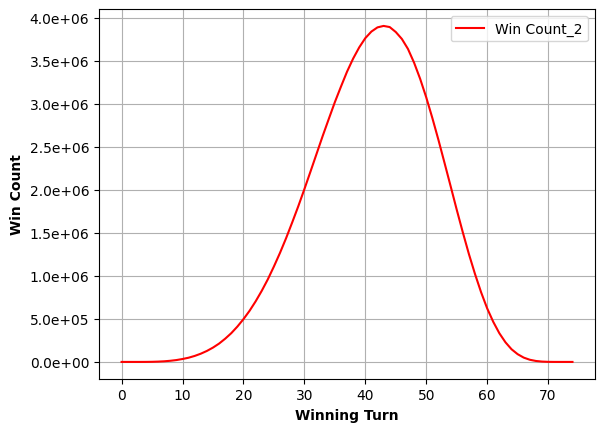
\includegraphics[scale=0.55]{../Dir_bingo_new/img_bingo2.png}
            \caption{2回目の当たる回数の分布}
            \label{img:bingo2}
          \end{center}
        \end{figure}
        \clearpage

        \subsubsection{3回目のシミュレーション結果}
        3回目のシミュレーション結果をグラフで表すと以下のグラフになる.
        \begin{figure}[htb]
          \begin{center}
            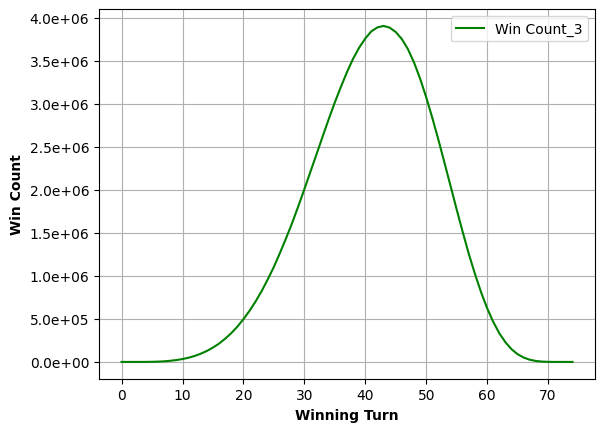
\includegraphics[scale=0.55]{../Dir_bingo_new/img_bingo3.png}
            \caption{3回目の当たる回数の分布}
            \label{img:bingo3}
          \end{center}
        \end{figure}

        \subsubsection{4回で当たる確率}
          各シミュレーションの結果から,4回で当たる確率は以下になる.
          \begin{itemize}
            \item シミュレーション1回目:$0.000345\%$
            \item シミュレーション2回目:$0.000318\%$
            \item シミュレーション3回目:$0.000339\%$
          \end{itemize}
        
        \subsubsection{7回で当たる確率}
          各シミュレーションの結果から,7回で当たる確率は以下になる.
          \begin{itemize}
            \item シミュレーション1回目:$0.012380\%$
            \item シミュレーション2回目:$0.012543\%$
            \item シミュレーション3回目:$0.012326\%$
          \end{itemize}
        
        \subsubsection{最も遅いゲームの回数}
          各シミュレーションの結果から,最も遅いゲームの回数は以下になる.
          \begin{itemize}
            \item シミュレーション1回目:$71$回
            \item シミュレーション2回目:$71$回
            \item シミュレーション3回目:$71$回
          \end{itemize}
        
        \subsubsection{最も遅いゲームが起こる確率}
          各シミュレーションの結果から,最も遅いゲームが起こる確率は以下になる.
          \begin{itemize}
            \item シミュレーション1回目:$0.000133\%$
            \item シミュレーション2回目:$0.000131\%$
            \item シミュレーション3回目:$0.000126\%$
          \end{itemize}
        
      \subsection{ビンゴのシミュレーションの考察}
      シミュレーションの結果から,以下のような結論が得られた.
      \begin{screen}
        \begin{itemize}
          \item 図(\ref{img:bingo1}),図(\ref{img:bingo2}),図(\ref{img:bingo3})から見ると,ビンゴになるまでの回数の分布は似ている.
          \item 4回以内で当たる確率は$0.0003\%$である.
          \item 7回以内で当たる確率は$0.012\%$である.
          \item 最も遅いゲームの回数は$71$回である.
          \item 最も遅いゲームが起こる確率は$0.00013\%$である.
        \end{itemize}
      \end{screen}

      % https://en.wikipedia.org/wiki/Probability

    \begin{thebibliography}{99}
      \bibitem{cite:rand}
      https://www.scaler.com/topics/random-number-generator-in-c/(参照2023-07-04)
      \bibitem{cite:wiki}
      https://en.wikipedia.org/wiki/Probability(参照2023-07-04)
    \end{thebibliography}

\end{document}